\documentclass[11pt, a4paper]{article}

% =============================================================================
%  1. ENCODING & LANGUAGE
% =============================================================================
\usepackage[utf8]{inputenc}      % UTF-8 source encoding
\usepackage[T1]{fontenc}         % 8-bit font encoding (correct hyphenation)
\usepackage{lmodern}             % Latin Modern scalable fonts
\usepackage[portuguese]{babel}   % Portuguese hyphenation & typography
\usepackage{csquotes}            % Context-sensitive quotation marks (best practice)

% =============================================================================
%  2. PAGE LAYOUT & TYPOGRAPHY
% =============================================================================
\usepackage[a4paper, margin=2.5cm]{geometry}
\usepackage{parskip}                      % Blank-line paragraph spacing; no indent
\usepackage[nopatch=footnote]{microtype}  % Micro-typographic refinements (kerning, tracking)
\usepackage{seqsplit}                     % Break long tokens at arbitrary points
\usepackage{float}                        % [H] float placement specifier
\setlength{\emergencystretch}{3em}        % Avoid overfull hboxes before giving up

% =============================================================================
%  3. MATHEMATICS
% =============================================================================
\usepackage{amsmath, amssymb}   % Extended math environments and symbols

% =============================================================================
%  4. COLORS
%  xcolor loaded with [table] BEFORE any \definecolor calls and other packages
% =============================================================================
\usepackage[table]{xcolor}

\definecolor{onoff}{RGB}{198, 239, 206}   % Light green – active On/Off cells
\definecolor{codebg}{RGB}{248, 248, 248}  % Near-white  – listing background
\definecolor{codekw}{RGB}{  0,   0, 180}  % Dark blue   – keyword highlight
\definecolor{codecm}{RGB}{  0, 128,   0}  % Dark green  – comment highlight
\definecolor{codestr}{RGB}{163,  21,  21} % Dark red    – string literal highlight

% =============================================================================
%  5. TABLES
% =============================================================================
\usepackage{array}      % Extended column specifications
\usepackage{booktabs}   % Publication-quality horizontal rules (\toprule etc.)
\usepackage{longtable}  % Tables that span multiple pages
\usepackage{tabularx}   % Auto-width X columns
\usepackage{multirow}   % Cells spanning multiple rows

% Convenience column types with explicit alignment
\newcolumntype{L}[1]{>{\raggedright\arraybackslash}p{#1}}
\newcolumntype{C}[1]{>{\centering\arraybackslash}p{#1}}

% =============================================================================
%  6. SYMBOLS
% =============================================================================
\usepackage{eurosym}   % \euro
\usepackage{pifont}    % Dingbats: \ding{55} = ✗,  \ding{51} = ✓

% =============================================================================
%  7. CODE LISTINGS
% =============================================================================
\usepackage{listings}

\lstdefinestyle{java}{
  language           = Java,
  % --- Portuguese accented characters inside listings ---
  literate           = %
    {á}{{\'{a}}}1  {à}{{\`{a}}}1  {ã}{{\~{a}}}1  {â}{{\^{a}}}1
    {é}{{\'{e}}}1  {ê}{{\^{e}}}1  {í}{{\'{i}}}1  {ó}{{\'{o}}}1
    {ô}{{\^{o}}}1  {õ}{{\~{o}}}1  {ú}{{\'{u}}}1  {ç}{{\c{c}}}1
    {Á}{{\'{A}}}1  {É}{{\'{E}}}1  {Í}{{\'{I}}}1  {Ó}{{\'{O}}}1
    {Ú}{{\'{U}}}1  {Ç}{{\c{C}}}1
    {º}{{\textordmasculine}}1  {ª}{{\textordfeminine}}1,
  % --- Base typography ---
  basicstyle         = \ttfamily\footnotesize,
  keywordstyle       = \color{codekw}\bfseries,
  commentstyle       = \color{codecm}\itshape,
  stringstyle        = \color{codestr},
  % --- Frame & background ---
  backgroundcolor    = \color{codebg},
  frame              = single,
  rulecolor          = \color{black!30},
  % --- Line numbers ---
  numbers            = left,
  numberstyle        = \tiny\color{black!60},
  numbersep          = 8pt,
  % --- Line breaking ---
  breaklines         = true,
  breakatwhitespace  = true,
  % --- Miscellaneous ---
  showstringspaces   = false,
  tabsize            = 2,
  captionpos         = b,
}

% =============================================================================
%  8. GRAPHICS & DIAGRAMS
% =============================================================================
\usepackage{graphicx}
\usepackage{tikz}
\usetikzlibrary{automata, positioning, arrows.meta, shapes.geometric, calc}

% =============================================================================
%  9. HYPERLINKS & CROSS-REFERENCING (Must be last)
% =============================================================================
\usepackage{hyperref}
\hypersetup{
  colorlinks  = true,
  linkcolor   = blue!60!black,
  urlcolor    = blue!60!black,
  citecolor   = blue!60!black,
  pdftitle    = {Second Project -- Report},
  pdfauthor   = {Dinis Rodrigues, Artur Krystopchuk, Gabriel Santos},
  pdfsubject  = {Software Testing and Validation},
  pdfkeywords = {software testing, boundary analysis, state machine, TestNG},
}

\usepackage[nameinlink, noabbrev]{cleveref} % Industry standard for cross-references
\crefname{table}{Table}{Tables}
\crefname{figure}{Figure}{Figures}
\crefname{section}{Section}{Sections}

% =============================================================================
%  CUSTOM COMMANDS
% =============================================================================

% --- Inline semantic markup ---
\newcommand{\code}[1]{\texttt{#1}}
\newcommand{\classname}[1]{\textsf{#1}}
\newcommand{\methodname}[1]{\texttt{#1()}}
\newcommand{\exn}[1]{\texttt{\seqsplit{#1}}}

% --- Result-tag annotations ---
\newcommand{\errtag}{\textcolor{red!70!black}{[error]}}
\newcommand{\singletag}{\textcolor{blue!70!black}{[single]}}
\newcommand{\boundarytag}{\textcolor{orange!80!black}{[boundary]}}

% --- Shared table formatting ---
\newcommand{\tablesettings}{%
  \setlength{\tabcolsep}{4pt}%
  \renewcommand{\arraystretch}{1.15}%
}

% =============================================================================
%  DOCUMENT METADATA
% =============================================================================
\title{%
  Software Testing and Validation \\[0.3em]
  \large Second Project --- Report%
}
\author{%
  Dinis Rodrigues (ist106213)   \and
  Artur Krystopchuk (ist104145) \and
  Gabriel Santos (ist1116334)%
}
\date{June 2026}

% =============================================================================
\begin{document}
% =============================================================================

\maketitle

\begin{abstract}
  This report presents the design of test cases for the urban delivery system described in the specification of the second project for the Software Testing and Validation course. Appropriate design strategies are applied to test the \classname{Order} and \classname{Delivery} classes at the class level, as well as the \methodname{computeDeliveryCost} and \methodname{updateItem} methods. The final section presents the TestNG implementation of eight selected test cases from the test suite of the \classname{Order} class.
\end{abstract}

\tableofcontents
\newpage

% =============================================================================
\section{Class-Level Testing of the \classname{Order} Class}
\label{sec:order-class}
% =============================================================================

\subsection{Chosen Strategy: Non-Modal Class Testing}
\label{sec:order-strategy}

The \classname{Order} class does not possess a state machine (there are no modes that alter method behaviour); its class-level behaviour is determined by a set of \emph{invariants} over its instance variables. The appropriate strategy for testing a class of this type is \textbf{Non-Modal Class Testing}, which consists of:
(i)~identifying the domains of the variables;
(ii)~determining the \emph{On}/\emph{Off} points for each invariant boundary; and
(iii)~constructing a \emph{domain matrix} with test vectors, where each test case exercises one boundary at a time, keeping the remaining variables at typical values.

\subsection{On/Off Points}
\label{sec:order-onoff}

\begin{longtable}{L{6.5cm} C{3.5cm} C{3.5cm}}
  \toprule
  \textbf{Boundary (invariant)} & \textbf{On} & \textbf{Off} \\
  \midrule
  \endfirsthead

  \multicolumn{3}{l}{\footnotesize\itshape (continuation of the previous table)} \\
  \toprule
  \textbf{Boundary (invariant)} & \textbf{On} & \textbf{Off} \\
  \midrule
  \endhead

  \midrule
  \multicolumn{3}{r}{\footnotesize\itshape (continues on the next page)} \\
  \endfoot

  \bottomrule
  \endlastfoot

  $\mathrm{client} \ne \code{null}$                             & Valid client        & \code{null}       \\
  $\mathrm{addr}   \ne \code{null}$                             & Valid string        & \code{null}       \\
  $\mathrm{addrLength} \ge 1$                                   & 1                   & 0 (empty)         \\
  $\mathrm{distance}   \ge 0$                                   & 0                   & $-1$              \\
  $\mathrm{distance}   \le 20000$                               & 20000               & 20001             \\
  $\mathrm{quantity}   \ge 1$                                   & 1                   & 0                 \\
  $\mathrm{quantity}   \le 10$                                  & 10                  & 11                \\
  $\mathrm{cost}       \le 1000$                                & 1000                & 1000.01           \\
  $\mathrm{totalQty}   \le 20 + \lfloor\mathrm{cost}/50\rfloor$ & $= \mathrm{limit}$ & $\mathrm{limit}+1$ \\
\end{longtable}

\subsection{Domain Matrix with Test Vectors}
\label{sec:order-matrix}

Each column represents a test case. In each column, exactly one boundary is in \emph{On} or \emph{Off} (shaded cell), while the remaining variables are at a typical value (row \emph{In}). Adopted typical value: order with one item of price $50$ and quantity $4$ ($\mathrm{cost}=200$, $\mathrm{totalQty}=4$, $\mathrm{limit}=24$), address length of $3$, and $\mathrm{distance}=5000$.

\begin{table}[H]
  \centering
  \small
  \tablesettings
  \caption{Domain matrix for the \classname{Order} class.}
  \vspace{0.2cm}
  \begin{tabularx}{\textwidth}{l l c *{10}{>{\centering\arraybackslash}X}}
    \toprule
    \textbf{Var.} & \textbf{Condition} & & \textbf{1} & \textbf{2} & \textbf{3} & \textbf{4} & \textbf{5} & \textbf{6} & \textbf{7} & \textbf{8} & \textbf{9} & \textbf{10} \\
    \midrule
    \multirow{3}{*}{addr}
      & \multirow{2}{*}{$\ge 1$}      & On  & \cellcolor{onoff}1 &                    &   &   &   &   &   &   &   &   \\
      &                               & Off &                    & \cellcolor{onoff}0 &   &   &   &   &   &   &   &   \\
      & Typical                       & In  &                    &                    & 3 & 3 & 3 & 3 & 3 & 3 & 3 & 3 \\
    \midrule
    \multirow{6}{*}{distance}
      & \multirow{2}{*}{$\ge 0$}      & On  &      &      & \cellcolor{onoff}0 &                       &                        &                        &      &      &      &      \\
      &                               & Off &      &      &                    & \cellcolor{onoff}$-1$ &                        &                        &      &      &      &      \\
      & \multirow{2}{*}{$\le 20000$}  & On  &      &      &                    &                       & \cellcolor{onoff}20000 &                        &      &      &      &      \\
      &                               & Off &      &      &                    &                       &                        & \cellcolor{onoff}20001 &      &      &      &      \\
      & Typical                       & In  & 5000 & 5000 &                    &                       &                        &                        & 5000 & 5000 & 5000 & 5000 \\
    \midrule
    \multirow{6}{*}{quantity}
      & \multirow{2}{*}{$\ge 1$}      & On  &   &   &   &   &   &   & \cellcolor{onoff}1 &                    &                     &                     \\
      &                               & Off &   &   &   &   &   &   &                    & \cellcolor{onoff}0 &                     &                     \\
      & \multirow{2}{*}{$\le 10$}     & On  &   &   &   &   &   &   &                    &                    & \cellcolor{onoff}10 &                     \\
      &                               & Off &   &   &   &   &   &   &                    &                    &                     & \cellcolor{onoff}11 \\
      & Typical                       & In  & 4 & 4 & 4 & 4 & 4 & 4 &                    &                    &                     &                     \\
    \midrule
    \multirow{3}{*}{cost}
      & \multirow{2}{*}{$\le 1000$}   & On  &     &     &     &     &     &     &    &   &     &     \\
      &                               & Off &     &     &     &     &     &     &    &   &     &     \\
      & Typical                       & In  & 200 & 200 & 200 & 200 & 200 & 200 & 50 & 0 & 500 & 550 \\
    \midrule
    \multirow{3}{*}{totalQty}
      & \multirow{2}{*}{$\le$ lim.}   & On  &   &   &   &   &   &   &   &   &    &    \\
      &                               & Off &   &   &   &   &   &   &   &   &    &    \\
      & Typical                       & In  & 4 & 4 & 4 & 4 & 4 & 4 & 1 & 0 & 10 & 11 \\
    \midrule
    \multicolumn{3}{l}{\textbf{Expected result}}
      & \checkmark & \ding{55} & \checkmark & \ding{55} & \checkmark & \ding{55}  & \checkmark & \ding{55} & \checkmark & \ding{55} \\
    \bottomrule
  \end{tabularx}
\end{table}

\begin{table}[H]
  \centering
  \small
  \tablesettings
  \caption{Domain matrix for the \classname{Order} class (continuation).}
  \vspace{0.2cm}
  \begin{tabularx}{\textwidth}{l l c *{8}{>{\centering\arraybackslash}X}}
    \toprule
    \textbf{Var.} & \textbf{Condition} & & \textbf{11} & \textbf{12} & \textbf{13} & \textbf{14} & \textbf{15} & \textbf{16} & \textbf{17} & \textbf{18} \\
    \midrule
    \multirow{3}{*}{client}
      & \multirow{2}{*}{$\ne$ \code{null}}  & On  &    &    &    &    & \cellcolor{onoff}ok &                              &    &    \\
      &                                     & Off &    &    &    &    &                     & \cellcolor{onoff}\code{null} &    &    \\
      & Typical                             & In  & ok & ok & ok & ok &                     &                              & ok & ok \\
    \midrule
    \multirow{3}{*}{addr}
      & \multirow{2}{*}{$\ne$ \code{null}} & On  &   &   &   &   &   &   & \cellcolor{onoff}"x" &                              \\
      &                                    & Off &   &   &   &   &   &   &                      & \cellcolor{onoff}\code{null} \\
      & typical length                     & In  & 3 & 3 & 3 & 3 & 3 & 3 &                      &                              \\
    \midrule
    distance & Typical                      & In  & 5000 & 5000 & 5000 & 5000 & 5000 & 5000 & 5000 & 5000 \\
    quantity & Typical                      & In  & ---  & ---  & ---  & ---  & ---  & ---  & ---  & ---  \\
    \midrule
    \multirow{3}{*}{cost}
      & \multirow{2}{*}{$\le 1000$}         & On  & \cellcolor{onoff}1000 &                          &     &     &     &     &     &      \\
      &                                     & Off &                       & \cellcolor{onoff}1000.01 &     &     &     &     &     &      \\
      & Typical                             & In  &                       &                          & 200 & 200 & 200 & 200 & 200 & 200  \\
    \midrule
    \multirow{3}{*}{totalQty}
      & \multirow{2}{*}{$\le$ lim.}         & On  &    &    & \cellcolor{onoff}24 &                     &   &   &   &   \\
      &                                     & Off &    &    &                     & \cellcolor{onoff}25 &   &   &   &   \\
      & Typical                             & In  & 20 & 20 &                     &                     & 4 & 4 & 4 & 4 \\
    \midrule
    \multicolumn{3}{l}{\textbf{Expected result}}
      & \checkmark & \ding{55} & \checkmark & \ding{55} & \checkmark & \ding{55} & \checkmark & \ding{55} \\
    \bottomrule
  \end{tabularx}
\end{table}

\noindent Legend: \checkmark{} = valid state (operation accepted); \ding{55}{} = invalid state (must throw \exn{InvalidOperationException} without changing the order state, according to I6).

\subsection{Relational Invariant (Same Supplier)}
\label{sec:order-i1}

This invariant is non-numeric, and therefore does not have On/Off points. It is tested with two dedicated cases:

\begin{longtable}{c L{8cm} L{4.5cm}}
  \toprule
  \textbf{\#} & \textbf{Scenario} & \textbf{Expected Result} \\
  \midrule
  \endfirsthead

  \multicolumn{3}{l}{\footnotesize\itshape (continuation)} \\
  \toprule
  \textbf{\#} & \textbf{Scenario} & \textbf{Expected Result} \\
  \midrule
  \endhead

  \bottomrule
  \endlastfoot

  19 & Add item from supplier $S$ to an order already containing items from supplier $S$  & Accepted (\checkmark) \\
  20 & Add item from supplier $S'$ to an order already containing items from supplier $S$ & \exn{InvalidOperationException} (\ding{55}) \\
\end{longtable}

% =============================================================================
\section{Class-Level Testing of the \classname{Delivery} Class}
\label{sec:delivery-class}
% =============================================================================

\subsection{State Machine}
\label{sec:delivery-fsm}

\begin{figure}[H]
  \centering
  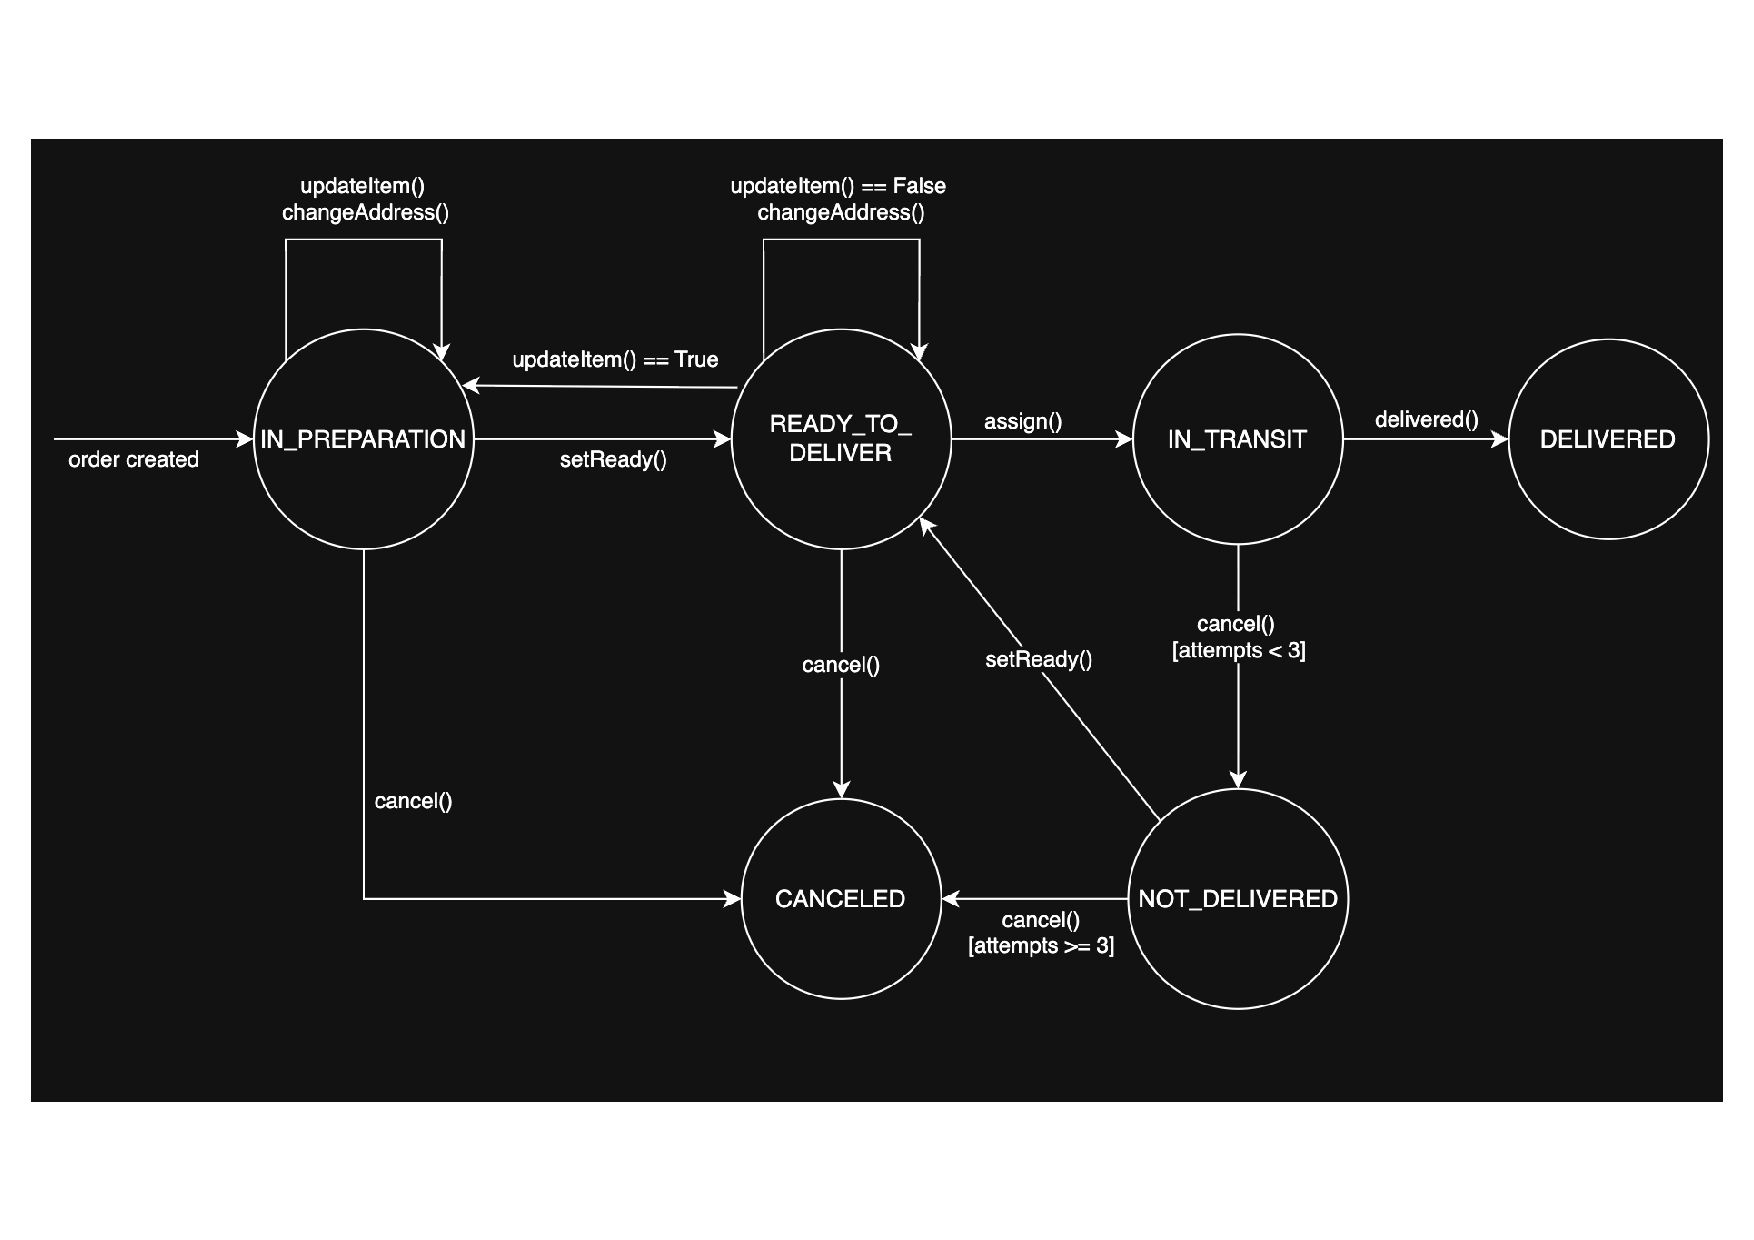
\includegraphics[width=\textwidth]{images/MaquinaEstados.pdf}
  \caption{State machine of the \classname{Delivery} class.}
  \label{fig:delivery-fsm}
\end{figure}

\subsection{Valid and Invalid Transitions}
% [TO FILL]
\textit{Transition table to be filled.}

\subsection{Strategy: \emph{Round-Trip / Transition Coverage}}
% [TO FILL]

\subsection{Test Cases}
% [TO FILL]

% =============================================================================
\section{Method \methodname{computeDeliveryCost}}
\label{sec:cdc}
% =============================================================================

\subsection{Strategy: Decision Table / Boundary Analysis}
% [TO FILL]

\subsection{Decision Table}
% [TO FILL]

\subsection{Test Cases}
% [TO FILL]

% =============================================================================
\section{Method \methodname{updateItem}}
\label{sec:updateitem}
% =============================================================================

\subsection{Chosen Strategy}
% [TO FILL]

\subsection{State + Input Combinations}
% [TO FILL]

\subsection{Test Cases}
% [TO FILL]

% =============================================================================
\section{Implementation in TestNG}
\label{sec:testng}
% =============================================================================

Four successful cases and four unsuccessful cases were selected from the test suite of the \classname{Order} class (\cref{sec:order-class}).

\begin{lstlisting}[
  style   = java,
  caption = {Skeleton of the TestNG test class for \classname{Order}.},
  label   = {lst:testng},
]
package supereats.tests;

import org.testng.annotations.*;
import static org.testng.Assert.*;

import supereats.core.*;

public class OrderTest {

  private static final double EPS = 1e-9;
  private Supplier s1;      // reference supplier
  private Supplier s2;      // distinct supplier
  private Client   client;
  // Items from supplier s1 (weight in grams, integer price)
  private Item i1;          // price 10
  private Item i2;          // price  5
  private Item i50;         // price 50 (for totalQty cases)

  // Item from a distinct supplier (s2)
  private Item iOther;

  @BeforeMethod
  public void setUp() {
    s1     = new Supplier("Loja A");
    s2     = new Supplier("Loja B");
    client = newClient();

    i1     = new Item(100,  10, s1, "Item 1");
    i2     = new Item(200,   5, s1, "Item 2");
    i50    = new Item(150,  50, s1, "Item 50");
    iOther = new Item(100,  10, s2, "Item from another supplier");
  }

  % Helper: the existence of a Client constructor is assumed.
  private Client newClient() {
    return new Client(/* ... valid data ... */);
  }

  // -------------------------------------------------------------------------
  // SUCCESS Cases
  // -------------------------------------------------------------------------

  // TC1: valid construction - all invariants satisfied.
  @Test
  public void tc1_validConstruction() {
    Order o = new Order(client, "Street A", 5000);

    assertEquals(o.totalQuantity(), 0);
    assertEquals(o.cost(), 0.0, EPS);
    assertTrue(o.itens().isEmpty());
  }

  // TC9: addItem in an empty order with a valid quantity.
  @Test
  public void TC9AddItemEmptyOrderValidQuantity() {
    Order o = new Order(client, "Street A", 5000);

    o.addItem(i1, 1);
    assertTrue(o.contains(i1));
    assertEquals(o.quantity(i1), 1);
    assertEquals(o.cost(), 10.0, EPS);
  }

  // TC13: boundary totalQty <= 20 + floor(cost/50) (On).
  // A unit price of 1 is used to isolate the totalQty boundary without
  // violating the cost limit (I3).
  // With cost = 24 * 1 = 24, the limit is
  // 20 + floor(24/50) = 20 + 0 = 20... therefore it is necessary to raise the
  // cost enough so that the limit reaches 24:
  //   limit = 24  <=>  floor(cost/50) = 4  <=>  cost in [200, 250).
  // Cost = 240 is chosen with items of price 10 (24 units * 10 = 240),
  // keeping cost <= 1000.
  @Test
  public void TC13TotalQuantityAtDynamicLimit() {
    Order o = new Order(client, "Street A", 5000);
    // 3 items of price 10, quantities 10 + 10 + 4 = 24 units
    Item a = new Item(150, 10, s1, "A");
    Item b = new Item(150, 10, s1, "B");
    Item c = new Item(150, 10, s1, "C");

    o.addItem(a, 10);
    o.addItem(b, 10);
    o.addItem(c,  4);

    assertEquals(o.totalQuantity(), 24); // = 20 + floor (240/50) = 24
    assertEquals(o.cost(), 240.0, EPS);
  }

  // TC19: adding an item from the SAME supplier is accepted.
  @Test
  public void TC19SameSupplierIsAccepted() {
    Order o = new Order(client, "Street A", 5000);

    o.addItem(i1, 2);
    o.addItem(i2, 3); // i2 also from supplier s1

    assertTrue(o.contains(i1));
    assertTrue(o.contains(i2));
    assertEquals(o.totalQuantity(), 5);
    assertEquals(o.cost(), 2 * 10 + 3 * 5, EPS);
  }

  // -------------------------------------------------------------------------
  // FAILURE Cases
  // -------------------------------------------------------------------------

  // TC2: boundary addrLength >= 1 (Off) - empty address.
  @Test(expectedExceptions = InvalidOperationException.class)
  public void TC2EmptyAddressThrows() {
    new Order(client, "", 5000);
  }

  // TC6: null client.
  @Test(expectedExceptions = InvalidOperationException.class)
  public void TC6NullClientThrows() {
    new Order(null, "Street A", 5000);
  }

  // TC10: boundary quantity <= 10 (Off) - quantity 11.
  @Test
  public void TC10QuantityAboveMaxThrowsAndKeepsState() {
    Order o = new Order(client, "Street A", 5000);
    try {
      o.addItem(i1, 11);
      fail("Expected InvalidOperationException");
    } catch (InvalidOperationException e) {
      assertFalse(o.contains(i1)); // state unchanged
      assertEquals(o.totalQuantity(), 0);
    }
  }

  // TC20: adding an item from a DISTINCT supplier.
  @Test(expectedExceptions = InvalidOperationException.class)
  public void TC20DifferentSupplierThrows() {
    Order o = new Order(client, "Street A", 5000);
    o.addItem(i1,     1); // supplier s1
    o.addItem(iOther, 1); // supplier s2 -> exception
  }
}
\end{lstlisting}

\end{document}
